%%%%%%%%%%%%%%%%%%%%%%%%%%%%%%%%%%%%%%%%%
% Journal Article
% Database System
% Practical 2: Analyze impact of storage format
%
% Gahan M. Saraiya
% 18MCEC10
%
%%%%%%%%%%%%%%%%%%%%%%%%%%%%%%%%%%%%%%%%%
%----------------------------------------------------------------------------------------
%       PACKAGES AND OTHER DOCUMENT CONFIGURATIONS
%----------------------------------------------------------------------------------------
\documentclass[paper=letter, fontsize=12pt]{article}
\usepackage[english]{babel} % English language/hyphenation
\usepackage{amsmath,amsfonts,amsthm} % Math packages
\usepackage[utf8]{inputenc}
\usepackage{float}
\usepackage{lipsum} % Package to generate dummy text throughout this template
\usepackage{blindtext}
\usepackage{graphicx} 
\usepackage{caption}
\usepackage{subcaption}
\usepackage[sc]{mathpazo} % Use the Palatino font
\usepackage[T1]{fontenc} % Use 8-bit encoding that has 256 glyphs
\usepackage{bbding}  % to use custom itemize font
\linespread{1.05} % Line spacing - Palatino needs more space between lines
\usepackage{microtype} % Slightly tweak font spacing for aesthetics
\usepackage[hmarginratio=1:1,top=32mm,columnsep=20pt]{geometry} % Document margins
\usepackage{multicol} % Used for the two-column layout of the document
%\usepackage[hang, small,labelfont=bf,up,textfont=it,up]{caption} % Custom captions under/above floats in tables or figures
\usepackage{booktabs} % Horizontal rules in tables
\usepackage{float} % Required for tables and figures in the multi-column environment - they need to be placed in specific locations with the [H] (e.g. \begin{table}[H])
\usepackage{hyperref} % For hyperlinks in the PDF
\usepackage{lettrine} % The lettrine is the first enlarged letter at the beginning of the text
\usepackage{paralist} % Used for the compactitem environment which makes bullet points with less space between them
\usepackage{abstract} % Allows abstract customization
\renewcommand{\abstractnamefont}{\normalfont\bfseries} % Set the "Abstract" text to bold
\renewcommand{\abstracttextfont}{\normalfont\small\itshape} % Set the abstract itself to small italic text
\usepackage{titlesec} % Allows customization of titles

\renewcommand\thesection{\Roman{section}} % Roman numerals for the sections
\renewcommand\thesubsection{\Roman{subsection}} % Roman numerals for subsections

\titleformat{\section}[block]{\large\scshape\centering}{\thesection.}{1em}{} % Change the look of the section titles
\titleformat{\subsection}[block]{\large}{\thesubsection.}{1em}{} % Change the look of the section titles
\newcommand{\horrule}[1]{\rule{\linewidth}{#1}} % Create horizontal rule command with 1 argument of height
\usepackage{fancyhdr} % Headers and footers
\pagestyle{fancy} % All pages have headers and footers
\fancyhead{} % Blank out the default header
\fancyfoot{} % Blank out the default footer

\fancyhead[C]{Institute of Technology, Nirma University $\bullet$ 25 September 2018} % Custom header text

\fancyfoot[RO,LE]{\thepage} % Custom footer text
%----------------------------------------------------------------------------------------
%       TITLE SECTION
%----------------------------------------------------------------------------------------
\title{\vspace{-15mm}\fontsize{24pt}{10pt}\selectfont\textbf{Practical 2: Analyze impact of storage format}} % Article title
\author{
\large
{\textsc{Gahan Saraiya, 18MCEC10 }}\\[2mm]
%\thanks{A thank you or further information}\\ % Your name
\normalsize \href{mailto:18mcec10@nirmauni.ac.in}{18mcec10@nirmauni.ac.in}\\[2mm] % Your email address
}
\date{}
\hypersetup{
	colorlinks=true,
	linkcolor=blue,
	filecolor=magenta,      
	urlcolor=cyan,
	pdfauthor={Gahan Saraiya},
	pdfcreator={Gahan Saraiya},
	pdfproducer={Gahan Saraiya},
}

\usepackage{makecell}

%----------------------------------------------------------------------------------------
\begin{document}
\maketitle % Insert title
\thispagestyle{fancy} % All pages have headers and footers

\newcommand*\tick{\item[\Checkmark]}
\newcommand*\arrow{\item[$\Rightarrow$]}
\newcommand*\fail{\item[\XSolidBrush]}

\section{Introduction}
\paragraph{}
The data can not be always considered to be fit in one size and the goal of this article is to deduce the impact of various storage format. 

Data needs to be stored in persistence storage, the focus is always to retrieve data efficiently.
To achieve that we need to have optimal storage mechanism/schemes that allows to access the data efficiently.   


\section{Static data placement on disk pages}
\subsection{N-ary Storage Model (NSM)}
	Also known as Slotted Page.
	\begin{itemize}
		\item record are stored sequentially on data pages
		\item Accesses full record (all attributes of record)
		\tick attributes of a same record are stored together
		\fail Doesn't work well on modern memory hierarchies
	\end{itemize}
	
	\paragraph{Flow}The whole page from disk is loaded in to main memory and then block(s) are fetched CPU cache
	\\
	\textbf{Impact}
	\begin{itemize}
		\tick Best results if full access to record is require
		\fail Partial record access is slow. Due to Fixed page layout it wastes I/O bandwidth
		\fail At CPU cache low spatial locality
	\end{itemize}

\subsection{Decomposition Storage Model (DSM)}
	Original Table is partitioned in to single attribute sub-tables.
	Each sub-table is stored in separate NSM page
	\begin{itemize}
		\item $N$-attribute table stored in to $N$ sub-tables
		\tick Saves I/O (eliminates unnecessary I/O)
		\fail Hard to modify/construct record afterwards
	\end{itemize}
	
	\paragraph{Flow} 
	Only required NSM page(s) (single attributed sub-table) is/are loaded in to main memory and blocks are fetched from loaded page
	\textbf{Impact}
	\begin{itemize}
		\tick Best results if partial access to record is require
		\fail full record access require reconstruction which may lead to unnecessary I/O and performance degraded compare to NSM
	\end{itemize}

\subsection{Partition Attribute Across (PAX)}
	In single page it partitions data for spacial locality by attribute
	\paragraph{Flow} 
	Likewise in NSM it loads whole PAX page from disk in to main memory. partitioned data are stored in to contiguous block and only require block(s) needs to be fetched
	\textbf{Impact}
	\begin{itemize}
		\tick Optimizes communication/transfer between Main memory and CPU cache memory (Increases Hit Ratio)
		\tick Optimal solution for both full and partial record access
	\end{itemize}

\section{Modern techniques of data storage}
Modern Data Storage techniques can be classified in below categories:
\begin{enumerate}
	\item Column-oriented DBMS
		\subitem stores data tables by column rather than by row
	\item Key-value pair
	\item Document oriented
	\item NoSQL (Not Only SQL database)
		\subitem not required to follow an established relational schema
	\item Graph Based
\end{enumerate}

\begin{figure}[H]
	\bgroup
	\setlength{\parindent}{-5em}
	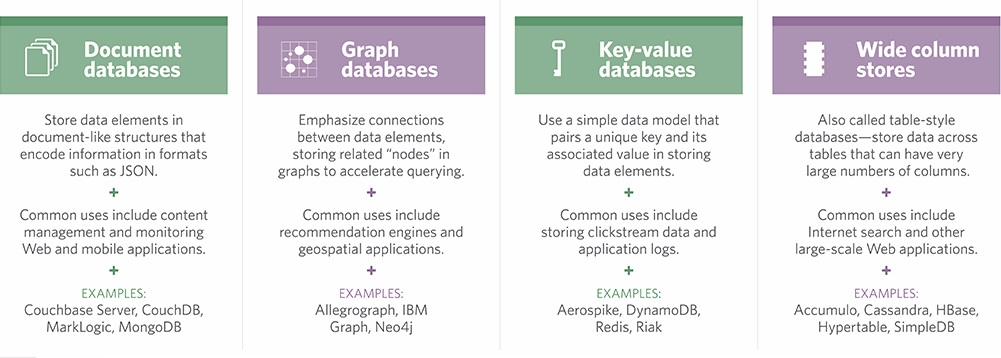
\includegraphics[width=550px]{refs/data_management-nosql.jpg}
	\egroup
	\caption{NoSQL family}
\end{figure}

%\begin{table}[H]
%	\bgroup
%	\setlength{\parindent}{-6em}
%	\def\arraystretch{2}%  1 is the default, change whatever you need
%	\begin{tabular}{c | c | c | c | c}
%		\thead{} 
%		& \thead{\large Document Oriented} 
%		& \thead{\large Graph based} 
%		& \thead{\large Key-Value Databases} 
%		& \thead{\large Column Oriented} 
%		\\ \hline \hline
%		Examples 
%		& \makecell{stores data elements in 
%			\\ document-like structures that 
%			\\ encode information in format 
%			\\ such as JSON} 
%		& \makecell{Emphasize connections 
%			\\ between data elements,
%			\\ storing related nodes in
%			\\ graphs to accelerate querying} 
%		& \makecell{Simple data model that pairs
%			\\ a unique key and its
%			\\ associated value in storing
%			\\ data elements} 
%		& \makecell{} \\
%	\end{tabular}
%	\egroup
%\end{table}

\subsection{Column-oriented DBMS}
	\paragraph{} stores data tables by column rather than by row.
	\begin{itemize}
		\item serializes all of the values of a column together
		\tick well suited for sparse data sets
		\fail retrieve all the data for a given record (entire row) requires more disk operations to collect data from multiple columns
	\end{itemize}
\subsection{Graph based}
	\begin{itemize}
		\tick easy to model and store relationship
		\tick performance of relationship traversal remains constant with growth in data size
		\tick queries are shortened and more readable
		\tick adding additional properties and relationship can be done on the fly - no migrations
	\end{itemize}
	
	\begin{figure}[H]
		\bgroup
		\setlength{\parindent}{-5em}
		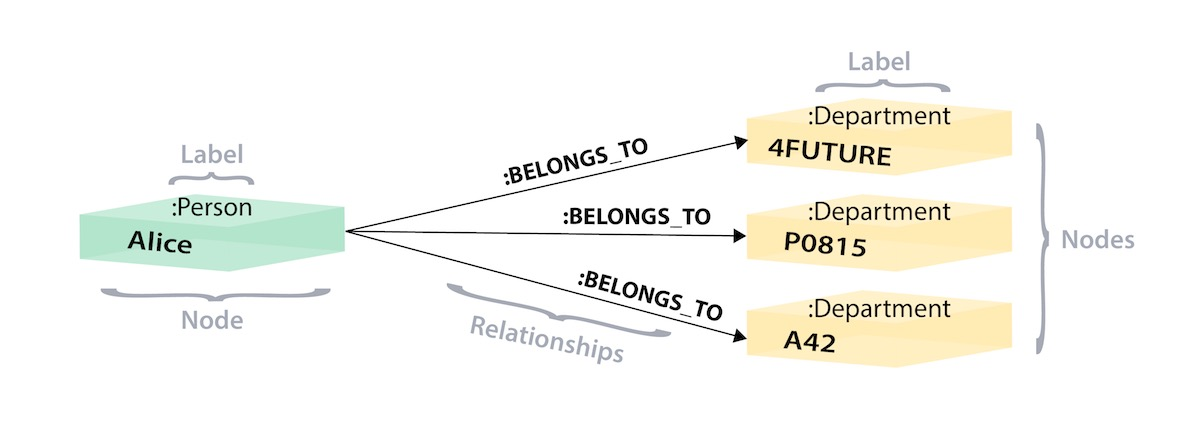
\includegraphics[width=550px]{refs/relational_graph_model.jpg}
		\egroup
		\caption{Graph – Alice and 3 Departments as nodes}
	\end{figure}


\section{Summary}


\setlength{\tabcolsep}{10pt} % Default value: 6pt
\renewcommand{\arraystretch}{1.5} % Default value: 1
\begin{table}[!ht]
\begin{flushleft}
\caption{Comparison of NSM, DSM and PAX}
\begin{tabular}{ l  c c c c }

\hline
{Performance} &\multicolumn{2}{ c }{\textbf{Cache$\leftrightarrow$Memory}} & \multicolumn{2}{ c }{\textbf{Memory$\leftrightarrow$Disk}}\\ 
\cline{1-5}
\textbf{Page Layout} & \textbf{full record access} & \textbf{partial record access} & \textbf{full-record access} & \textbf{partial record access} \\
\hline
NSM & \CheckmarkBold & \XSolidBrush & \CheckmarkBold & \XSolidBrush \\ 
DSM & \XSolidBrush & \CheckmarkBold & \XSolidBrush & \CheckmarkBold \\ 
PAX & \CheckmarkBold & \CheckmarkBold & \CheckmarkBold & \XSolidBrush \\ 
 \hline
\end{tabular}
\end{flushleft}
\end{table}


%----------------------------------------------------------------------------------------
%\end{multicols}
\end{document}
